\documentclass[10.5pt]{article}
\usepackage[a4paper,margin=2.2cm]{geometry}
\usepackage{fontspec}
\setmainfont{texgyrepagella}[Extension=.otf,UprightFont=*-regular,BoldFont=*-bold,ItalicFont=*-italic,BoldItalicFont=*-bolditalic]
\setsansfont{texgyreheros}[Extension=.otf,UprightFont=*-regular,BoldFont=*-bold,ItalicFont=*-italic,BoldItalicFont=*-bolditalic,Scale=0.92]
\usepackage{graphicx,booktabs,tabularx,xcolor,titlesec,enumitem,caption,float}
\usepackage[most]{tcolorbox}
\usepackage{xurl}
\usepackage[hidelinks]{hyperref}
\definecolor{accent}{HTML}{C0392B}\definecolor{ink}{HTML}{1F2A36}\definecolor{soft}{HTML}{F6F1EE}
\titleformat{\section}{\sffamily\large\bfseries\color{ink}}{}{0pt}{}
\titleformat{\subsection}{\sffamily\normalsize\bfseries\color{accent}}{}{0pt}{}
\titlespacing*{\section}{0pt}{12pt}{4pt}\titlespacing*{\subsection}{0pt}{8pt}{2pt}
\captionsetup{font={small,it},labelformat=empty,skip=4pt}
\setlist[itemize]{leftmargin=1.2em,itemsep=2pt,topsep=3pt}
\setlength{\parskip}{4pt}\setlength{\parindent}{0pt}
\linespread{1.06}\emergencystretch=3em
\begin{document}
\begin{center}
{\sffamily\bfseries\LARGE\color{ink} The Notes That Vanish: Self-Deletion Inflates AI Fact-Checkers' Track Record on X\par}
\vspace{8pt}
{\large Malyadri Chowdary Marneni¹, Poojitha G², Chandana R³\par}
{\small\itshape ¹Student researcher, Masters' Union University\\²Sapthagiri NPS University; Research intern, Indian Institute of Management Bangalore\\³BGS College\par}
\vspace{2pt}{\footnotesize AI x Epistemics Research Sprint, Apart Research, November 2026\par}
\end{center}
\vspace{4pt}
\begin{tcolorbox}[colback=soft,colframe=soft,boxrule=0pt,arc=2pt,left=10pt,right=10pt,top=6pt,bottom=6pt]
{\sffamily\bfseries\color{accent} Abstract}\par\small Roughly one in six Community Notes written by AI on X quietly disappears. AI writers now draft about half of all new notes, and published comparisons score them by how often raters mark their surviving notes Helpful. This pre-registered audit measures what that score cannot see. Using X's public record of notes from September 2025 to October 2026 (369,568 AI and 823,110 human notes), AI writers deleted 17.3\% of their notes against 6.8\% for humans. Nearly all of these deletions come from seven accounts, six of them high-volume, and jump in April 2026, a pattern consistent with the automatic deletion of likely failures that X describes in its own AI writer. Counting the deleted notes halves the AI advantage in reaching Helpful status, from +4.3 to +2.2 points, a clear shrinkage but below our pre-registered 5-point margin, and one that may rest on a single operator. Three LLM judges from different vendors checked the pages cited by 800 AI and human notes on the same 400 posts; none called any of 150 deliberately mismatched pages support, though they caught few notes with one number altered. AI notes cited a readable source far more often and, among notes with a readable source, were unsupported no more often than human notes (4.7\% vs 9.3\%, difference not statistically clear). Whether raters' own source tags track support could not be settled. Evaluations of AI fact-checkers should count deleted notes, and their sources show no detectable gap against human notes (provisional).
\end{tcolorbox}

\begin{tcbraster}[raster columns=3,raster equal height,raster column skip=6pt]\begin{tcolorbox}[colback=white,colframe=accent!60,boxrule=0.5pt,arc=2pt,halign=center,top=4pt,bottom=4pt]{\sffamily\bfseries\Large\color{accent} 17.3\% vs 6.8\%}\par\vspace{1pt}{\footnotesize of notes deleted by AI vs human writers}\end{tcolorbox}\begin{tcolorbox}[colback=white,colframe=accent!60,boxrule=0.5pt,arc=2pt,halign=center,top=4pt,bottom=4pt]{\sffamily\bfseries\Large\color{accent} +4.3 → +2.2}\par\vspace{1pt}{\footnotesize AI advantage in reaching Helpful, before and after counting deletions (points)}\end{tcolorbox}\begin{tcolorbox}[colback=white,colframe=accent!60,boxrule=0.5pt,arc=2pt,halign=center,top=4pt,bottom=4pt]{\sffamily\bfseries\Large\color{accent} 4.7\% vs 9.3\%}\par\vspace{1pt}{\footnotesize of AI vs human Helpful notes with an unsupporting source}\end{tcolorbox}\end{tcbraster}
\section*{1. Introduction}
If a student could erase every test they were about to fail, their grade point average would look excellent. That is, in effect, the position of some AI fact-checkers on X today.

Community Notes is X's crowd-sourced fact-checking system: contributors propose notes on posts, and a note is shown to everyone only when raters who usually disagree both rate it Helpful. Since September 2025, AI programs can write notes through an API on the same terms as people, and they now draft about half of all new notes (Figure 2). Meta, TikTok and YouTube have adopted or trialled similar systems, so whether AI fact-checkers can be trusted at scale is becoming a question about the information diet of billions of people.

So far the answer has come from one number: how often raters mark AI notes Helpful. By that measure AI writers look strong, beating ordinary contributors [1, 2, 3]. But the number has two blind spots. It is computed on the notes that survive, and X's own paper on its AI writer describes a model that deletes notes predicted to fail after as few as three ratings [4]. And it measures whether a note persuades raters, not whether the sources it cites say what it claims. Raters are not required to open those sources. A fact-checker that sounds right but cites pages that do not back it up would pass this test, which is exactly the failure an epistemic system most needs to catch.

Forecasters will recognise the first problem. A Helpful rate computed on surviving notes behaves like an improper score: like a forecaster allowed to delete predictions before they resolve, a writer can raise it by withdrawing likely failures, without becoming any more accurate. Formally, if each note would reach Helpful with probability p and the writer deletes, before rating, every note whose p is below a threshold t, the surviving-note rate becomes the average p among kept notes, which rises with t although no note improves. The rate over all submitted notes, with deleted notes counted as not Helpful, cannot be raised by deleting, so it removes the incentive.

This project audits AI fact-checkers on both blind spots, independently of the platform's own scoring, with every hypothesis fixed in advance. Its contributions:

\begin{itemize}
\item A survivorship correction on the full public record (1,192,678 notes). AI writers delete notes 2.5 times as often as humans, almost entirely through six large accounts, and counting those deletions halves their advantage in reaching Helpful status.
\item A source audit of 800 AI and human notes on the same 400 posts, using three LLM judges from different vendors, a deterministic quote check and a mismatched-page control. AI notes cite readable sources more often and are not more often unsupported among notes with a readable source.
\item Evidence that LLM source-checkers reject off-topic pages but catch few altered details: with one number changed in notes all judges had called supported, any judge flagged only 23 of 62.
\item A test of whether raters' source tags track verified support (inconclusive), plus a per-writer reliability table and a one-command script that rebuilds every number from any day's public data.
\end{itemize}
\begin{table}[htbp]\centering\small\renewcommand{\arraystretch}{1.25}\begin{tabularx}{\linewidth}{@{}>{\raggedright\arraybackslash}X>{\raggedright\arraybackslash}X>{\raggedright\arraybackslash}X@{}}\toprule
\textbf{\sffamily Pre-registered question} & \textbf{\sffamily Result (AI minus human)} & \textbf{\sffamily Verdict}\\\midrule
H1. Does counting deleted notes shrink the AI advantage in reaching Helpful? & Shrinkage +2.2 points [+1.6, +2.4]: advantage falls from +4.3 to +2.2 & Supported in direction (p < 0.001); below the 5-point margin\\
H2. Do AI and human notes differ in how often they lose Helpful status? & −1.3 points [−2.5, −0.1], same posts & No clear difference (p = 0.07); inside the 5-point margin\\
H3. Do AI and human notes differ in how often a cited source fails to support them? & −4.6 points [−9.8, +0.6] & No detectable difference (p = 0.17); provisional (D9)\\
H4. Are raters' ``good sources'' tags blind to whether sources support the note? & +3.8 points [−1.4, +8.9], supported minus unsupported & Inconclusive: too few unsupported notes\\
\bottomrule\end{tabularx}\caption{Table 1. The four pre-registered hypotheses at a glance. Brackets: 95\% bootstrap intervals. p-values are normal approximations from the bootstrap standard error, Holm-corrected across the four tests as planned.}\end{table}
\section*{2. Related Work}
Gong and Wu [1] characterise 20 AI writers and find their notes are rated helpful less often than expert human notes but more often than laypeople's. Li and Bakker [2] ran an LLM writer in the field and compared its 1,614 notes with human notes on the same posts; the LLM notes received more positive ratings across political viewpoints. R Street [3] analysed seven months of public data and reported that AI notes reached Helpful status at 18.0\% against 8.9\% for human notes, using data up to March 2026; that window ends as AI deletion begins (Figure 2), and its writer set and outcome definition also differ from ours, which may explain why its gap is larger than the one reported here. X's engineers [4] describe the API, the earn-in and quota rules, and their own Community Writer, including a Deletion Model that ``identifies notes that are unlikely to obtain CRH status and proactively deletes the notes'' after as few as three ratings. De et al. [5] study collaborative notes drafted by an LLM and refined by human feedback. Earlier work examines whether Community Notes reduce engagement with misleading posts [6], what threatens contributor participation [7], and how the system evolved over four years [8]. A recent survey of AI for epistemics names Community Notes as a prime example of deployed epistemic infrastructure [9].

All AI-versus-human comparisons above score notes by rater outcomes. None of them, as far as their abstracts and reported methods show, accounts for notes their writers deleted, and none checks whether cited sources support the notes. This project adds both measures and uses the platform's own rating tags as a comparison rather than as ground truth.

\section*{3. Methods}
The hypotheses, definitions, sample size, judge design and analysis were written down and committed before any outcome data was read (PREREG.md, first commit of the repository). Every later change is logged with its reason in DEVIATIONS.md (nine entries, covering judge substitutions forced by missing credit, usage limits and API errors, and the reduced human check described below).

\subsection*{Data and definitions (Part 1)}
We used X's public Community Notes release of 14 November 2026: the note, note-status-history and user-enrolment files. The window is notes created from 2 September 2025 (first AI writer admitted) to 31 October 2026. An AI note is one whose author is enrolled as an API writer (39 writers with notes in the window). One account that writes collaborative notes (55,917 notes) is analysed separately. The status-history file keeps every note ever created, while the notes file drops deleted ones, so a note present in the first and absent from the second counts as deleted by its author. A note is ever Helpful if it reached Currently Rated Helpful (CRH) at any point, and has lost Helpful if it was ever CRH but is not now. Intervals are author-cluster bootstraps (2,000 resamples, fixed seed) for group differences and Wilson intervals for single rates.

H1 (survivorship) compares the AI-minus-human difference in ever-Helpful rate computed on surviving notes only, as published comparisons do, with the same difference on all notes. H2 (reversal) compares how often ever-Helpful notes lose that status, within posts that have both an AI and a human ever-Helpful note (5,487 posts). The smallest effect of interest was fixed at 5 points.

\subsection*{Citation audit (Part 2)}
The sample is 400 posts drawn by hash order from posts with both an AI and a human note that reached Helpful status, one note of each kind per post (800 notes, 1,575 cited links). Each link was fetched live, with an Internet Archive copy as fallback. Links to social-media and video sites, login walls and pages that block automated access were marked uncheckable rather than judged; dead links were recorded as such. This left 779 readable note-page pairs.

Each pair was judged with one frozen prompt that asks whether the cited page supports the note's main factual claim (SUPPORTS, PARTIAL, DOES\_NOT\_SUPPORT or UNCHECKABLE) and requires a verbatim supporting quote. Judges never see whether a note is AI or human. A deterministic check, fixed before judging, demotes any support label whose quote is not found on the page. Judge A is Claude Sonnet 5.5 and Judge B is Qwen 3.5 397B; Judge C, GLM 5.2, is used only for robustness. A note is unsupported if any readable cited page does not support it. The primary estimate uses notes on which Judges A and B agree; lower and upper bounds count notes both, or either, call unsupported.

Two checks test the judges. In a negative control, 150 notes were each paired with a readable page cited by a note on a different post; a sound judge should almost never call such a page support. An earlier run of GPT-5.6 on 110 pairs, stopped by a usage limit, gives an extra agreement check. A harder control, added during the sprint (DEVIATIONS D8), takes pairs that all three judges called supported, changes one number in the note (years by three, other numbers by half again) and asks whether the judges notice that the page no longer backs it. Finally, two authors independently hand-labelled 106 links from 60 notes, half drawn at random and half from notes Judge A flagged, without seeing which was which or each other's labels (DEVIATIONS D7).

\subsection*{Rater blindness (Part 3)}
For the same notes we took all 90,742 public ratings and computed, per note, the share of raters who ticked ``good sources'' and the share who ticked ``sources missing or unreliable''. H4 asks whether these shares differ between notes the judges agree are supported and notes they agree are unsupported, with ±5 points as the equivalence margin.

\section*{4. Results}
\begin{tcolorbox}[colback=white,colframe=accent,boxrule=0.6pt,arc=2pt,left=8pt,right=8pt,top=5pt,bottom=5pt]\small{\sffamily\bfseries\color{accent} Results in brief.} (1) Counting deleted notes halves the AI advantage in reaching Helpful status; the effect comes from six accounts that delete about a fifth of their notes. (2) Once Helpful, AI notes keep that status as well as human notes. (3) Among notes with a readable source, AI notes are not more often unsupported, but this rests on LLM judges that agree only moderately with human labels (two human labellers agreed no better with each other) and miss altered details. (4) Whether raters' source tags track support could not be settled.\end{tcolorbox}
\subsection*{Part 1: deletion flatters AI writers' track record}
\begin{figure}[htbp]\centering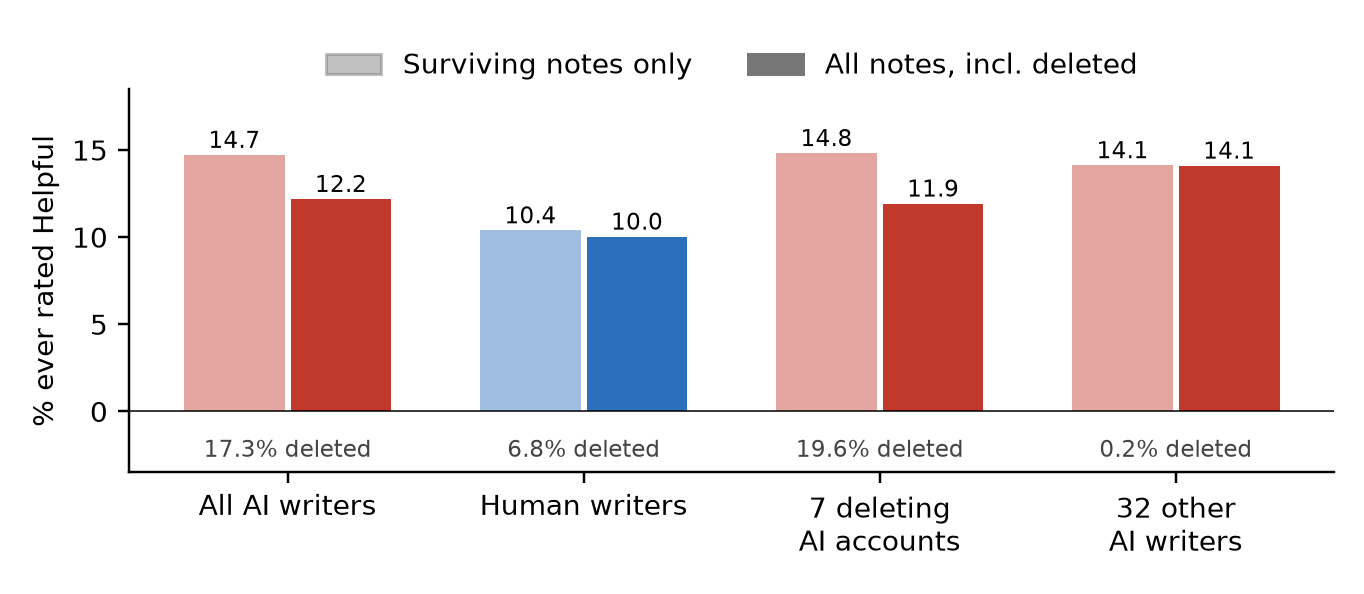
\includegraphics[width=\linewidth]{../results/fig1_survivorship.png}\caption{Figure 1. Share of notes ever rated Helpful, on surviving notes (light) and on all notes including deleted ones (dark), for notes created 2 Sep 2025 to 31 Oct 2026 (369,568 AI, 823,110 human). Below each group: share deleted by the author. The 7 deleting accounts look best on surviving notes and worst once deletions count. All 95\% Wilson intervals have half-widths under 0.4 points.}\end{figure}
AI writers deleted 17.3\% of their notes; human writers deleted 6.8\% (Figure 1). On surviving notes, AI notes reached Helpful status more often than human notes, +4.3 points [95\% CI +3.6, +5.1]. Counting deleted notes, the advantage is +2.2 points [95\% CI +1.6, +3.1]. H1 is supported: the shrinkage is +2.2 points [95\% CI +1.6, +2.4] (p < 0.001, Holm-corrected), about half of the headline advantage, although it falls short of the 5-point smallest effect of interest fixed in advance.

Counting deleted notes is the like-for-like comparison. A human note that fails stays in the record as not Helpful and counts against its writer; an AI note withdrawn before its verdict would otherwise vanish from the denominator. Counting it treats both kinds of writer the same way, which is also how X's quota system scores AI writers [4].

Once Helpful, AI notes keep that status no worse than human notes. Within the 5,487 posts with both kinds of ever-Helpful note, 12.6\% of AI notes and 14.0\% of human notes later lost it, a difference of −1.3 points [95\% CI −2.5, −0.1]. The difference is small and, after the planned Holm correction, not statistically significant (p = 0.07); either way it is far inside the 5-point margin, so AI notes are no less stable once Helpful. Across all notes the raw rates differ more (13.0\% vs 18.0\%), but human notes are older and on different posts; reweighting human notes to the AI notes' months still leaves a −7.7-point gap. The same-post comparison, the pre-registered primary, removes most of that confounding.

\subsection*{Part 1, exploratory: who deletes, and what deleted notes would have scored}
The deletions are not spread across AI writers. 7 accounts delete more than 5\% of their notes; together they wrote 88\% of AI notes and deleted 19.6\% of them, while the other 32 AI writers deleted 0.2\%. AI deletion was near zero until February 2026, rose in March and jumped to 15 to 22\% a month from April (Figure 2), which fits a deletion policy being switched on rather than a gradual change in writing. This pattern matches the Deletion Model in X's Community Writer [4], although hashed ids mean the accounts cannot be named. On surviving notes the deleting accounts look slightly better than the other AI writers (14.8\% vs 14.1\% ever Helpful); on all notes they look worse (11.9\% vs 14.1\%).

\begin{figure}[htbp]\centering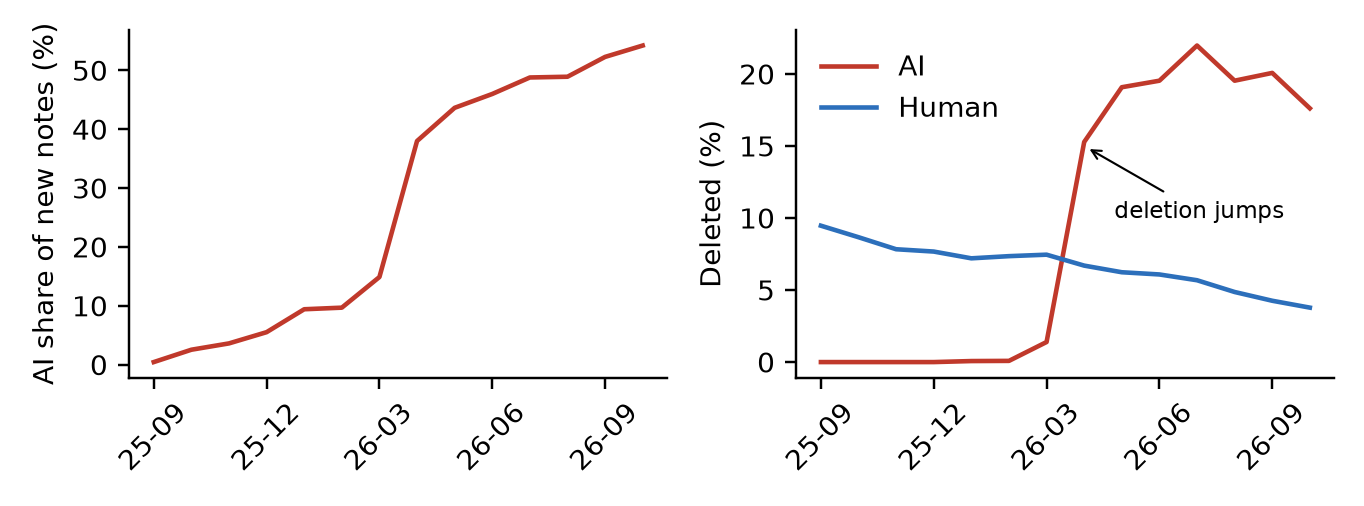
\includegraphics[width=\linewidth]{../results/fig2_monthly.png}\caption{Figure 2. Left: AI writers' share of new notes by month. Right: share of each month's notes later deleted by their author. AI deletion rises in March 2026 and jumps from April. Recent months have had less time for notes to be deleted, which may explain part of the fall in the human line; X's deletion model can act as soon as three ratings arrive [4].}\end{figure}
Why the advantage shrinks matters more than the fact that it does. Only 0.07\% of the notes AI writers deleted had ever been rated Helpful, against 5.1\% of the notes humans deleted. AI notes are withdrawn before raters reach a verdict, so their outcome is never observed. The two published-style comparisons therefore bracket the truth. Counting deleted notes as failures, as X's own quota rules do [4], gives the lower bound; counting only surviving notes assumes deleted notes would have done as well as the rest, which a deletion model aimed at likely failures makes implausible. If deleted AI notes would have reached Helpful at a quarter of the surviving rate, the advantage would be +2.8 points; at half, +3.4. The headline +4.3 requires deleted notes to be at least as good as surviving ones.

The effect belongs to a design, not to AI writers in general (Table 2). Without the deleting accounts the shrinkage disappears, and the other AI writers lead humans even with deleted notes counted. Six of the deleting accounts look alike (53,000 to 55,000 notes each, starting in November or December 2025, 19 to 20\% deleted) and may be one operator; the seventh is a 77-note account just over the 5\% cutoff. Treated as one cluster, the shrinkage interval spans zero, because the population then holds effectively one deleter. Notes with at least ten weeks of follow-up give the same shrinkage.

\begin{table}[htbp]\centering\small\renewcommand{\arraystretch}{1.25}\begin{tabularx}{\linewidth}{@{}>{\raggedright\arraybackslash}X>{\raggedright\arraybackslash}X>{\raggedright\arraybackslash}X@{}}\toprule
\textbf{\sffamily Analysis} & \textbf{\sffamily Shrinkage, points} & \textbf{\sffamily AI minus human, all notes}\\\midrule
Pre-registered: each writer a cluster & +2.2 [+1.6, +2.4] & +2.2 [+1.6, +3.1]\\
Deleting accounts as one cluster & +2.2 [−0.4, +2.5] & +2.2 [+1.7, +6.7]\\
Without the 7 deleting accounts & −0.3 [−0.4, −0.3] & +4.1 [+1.3, +7.6]\\
Notes created to August 2026 & +2.1 [+1.5, +2.4] & +2.5 [+1.7, +3.9]\\
\bottomrule\end{tabularx}\caption{Table 2. H1 under exploratory checks (rows 2 to 4 not pre-registered). Brackets: 95\% author-cluster bootstrap intervals; they are asymmetric because six accounts hold 88\% of AI notes, so each resample depends on how often they are drawn.}\end{table}
\subsection*{Part 2: no detectable gap in whether sources support the notes}
AI notes cited a readable source far more often: 54\% of AI-cited links could be read and judged against 44\% of human-cited links, and 53.2\% of human notes had no checkable source at all, against 33.0\% of AI notes. Human notes lean more on posts, videos and other social-media links. Dead links were rare in both groups (2.8\% vs 2.5\% of notes).

\begin{figure}[htbp]\centering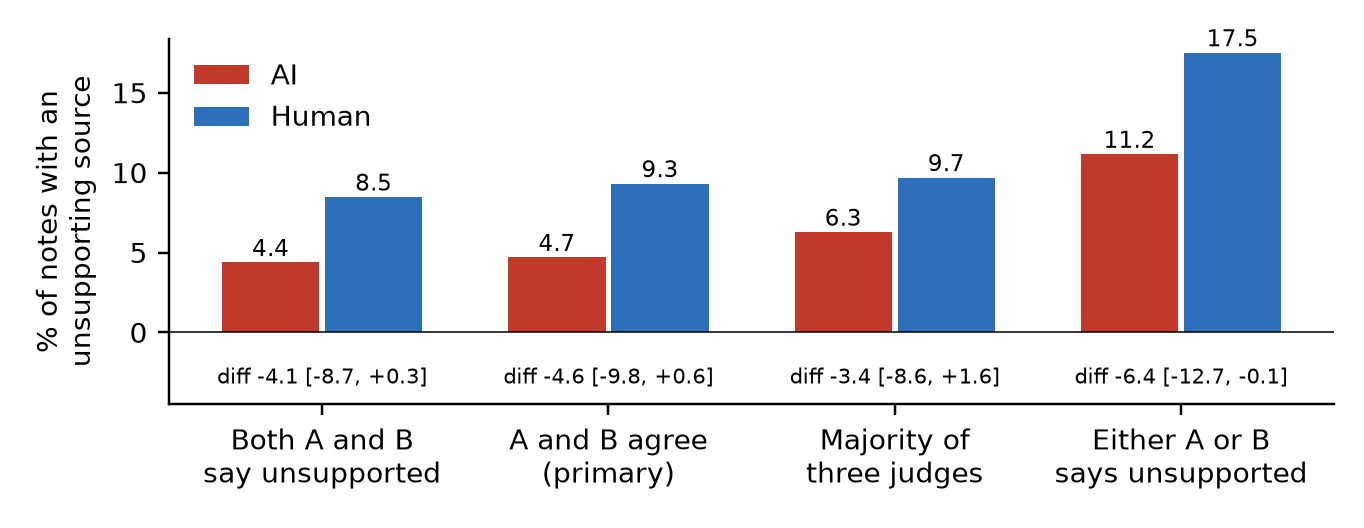
\includegraphics[width=\linewidth]{../results/fig3_support.png}\caption{Figure 3. Share of notes with at least one readable cited page that does not support the note, under four judge rules. Below each pair: AI minus human, points, with 95\% post-cluster bootstrap interval. Under every rule the point estimate favours AI notes; only under the loosest rule does the interval exclude zero.}\end{figure}
Among notes with a readable source, AI notes were not more often unsupported (Figure 3). On the primary measure, notes where Judges A and B agree, 4.7\% of AI notes and 9.3\% of human notes were unsupported (234 and 161 notes), a difference of −4.6 points [95\% CI −9.8, +0.6]. The bounds and the majority of three judges point the same way, and in 113 same-post pairs where both notes were judged, only the AI note was unsupported in 2 pairs and only the human note in 8 (two-sided sign test p = 0.11). H3 finds no detectable difference (p = 0.17, Holm-corrected); if anything, the data lean towards AI notes being better sourced. The sample could reliably detect a difference of about 7 points, so smaller gaps in either direction cannot be ruled out; the result is ``no worse'', not ``better''.

Three exploratory checks probe H3. The sign does not depend on the judge: used alone, Judges A, B and C give −4.1, −6.8 and −3.3 points. In the hand-labelled links there is no sign that judges are more lenient towards AI notes: of the links the first author called unsupported, Judge C passed 5 of 8 AI-cited and 11 of 15 human-cited links, if anything more lenient towards human notes, but too few for a test. Coverage is the real limit. Using Judge A alone, over all 800 notes it finds 19 AI and 21 human notes unsupported, while 132 AI and 213 human notes have no checkable source. If those notes are unsupported at the same rate in both groups, AI notes never come out worse; but if only AI notes' unreadable sources were bad, a rate of 1.5\% among them would close the gap. H3 holds for notes with readable sources and says nothing about the rest.

The judges passed the negative control: none of the three called any of the 150 mismatched pages support (Judge A 0, Judge B 0, Judge C 0). Agreement between Judges A and B on real pairs was moderate (Cohen's kappa 0.43 per link, 0.57 per note). The largest group of disagreements (95 of 234) was PARTIAL against SUPPORTS; only 6 were support against no support. On the 110 GPT-5.6 pairs, kappa with Judges A, B and C was 0.60, 0.58 and 0.52.

Against the first author's hand labels on 106 links from 60 notes (DEVIATIONS D7), kappa was 0.51 for Judge A, 0.40 for Judge B and 0.32 for Judge C, and 0.37, 0.30 and 0.22 on the random half alone. The first author called 23 links unsupported. Of the 35 Judge A called unsupported, 20 were also unsupported to the first author, who rated the other 15 PARTIAL (8) or uncheckable (7), never clear support. The judges lean lenient, not harsh: Judge C called 16 of the 23 links the first author called unsupported supported or partly supported, Judge B 6 and Judge A 1 (Judge A's figure is flattered, since half the sheet was chosen from its flags). The H3 rates are therefore best read as lower bounds, and the judges are weakest exactly where a fact-checker most needs them.

The task is hard for humans too. The second author labelled the same links independently; the two agreed on 50 of 106 (kappa 0.29; 0.21 on the random half), rising to 0.46 when only ``does not support'' is separated from everything else, the distinction H3 rests on. The commonest disagreement (20 links) was the first author's SUPPORTS against the second's PARTIAL. Judge A agrees with the first author more closely than the two authors agree with each other, while all three judges agree less with the stricter second author (0.12 to 0.25, and near zero on the random half). Against the pre-registered human consensus, the 50 links both authors labelled alike, kappa was 0.48, 0.42 and 0.26 for Judges A, B and C.

This triggers a pre-registered gate. PREREG section 6 says that if judge-human kappa at note level is below 0.60, H3 and H4 are reported on the human-labelled set only. Note-level kappa against the first author was 0.56, 0.44 and 0.30 for Judges A, B and C on all 60 notes, and 0.00, 0.21 and −0.06 on the random half, where a single unsupported note makes kappa close to meaningless. Against the two authors' consensus the per-link figures above are also below 0.60. The human-labelled set is too small to test anything: in its random half, 0 of 23 AI notes and 1 of 7 human notes were unsupported to the first author, in line with the judge result but with no power. We therefore keep the judge-based H3 and H4 in the main text and mark them provisional (DEVIATIONS D9).

The harder control exposes the judges' limit. In 62 pairs where one number in the note was changed and the new number appears nowhere on the page, Judge A flagged 4, Judge B 15 and Judge C 15; at least one judge flagged 23. Their reasons show why: they check whether the page backs the note's main point and pass over wrong dates and figures. The citation results above therefore measure whether sources support what a note is about, not whether every detail is right; detail errors are largely invisible to this method, for AI and human notes alike.

\begin{tcolorbox}[colback=white,colframe=accent,boxrule=0.6pt,arc=2pt,left=8pt,right=8pt,top=5pt,bottom=5pt]\small{\sffamily\bfseries\color{accent} What an unsupported Helpful note looks like.} An AI note said an image showed the 2003 breakup of Space Shuttle Columbia, not Artemis 2, and cited a NASA Ames page; the page is a general overview of the division that never mentions Columbia. A human note called viral ``hero dog'' rescue clips AI-generated and cited a 2021 National Geographic article, which is about staged rescues using real animals, not AI. Both notes reached Helpful status; in both, the claim may well be true, but the cited source does not show it. Both judges agreed on each case.\end{tcolorbox}
\subsection*{Part 3: do raters' source tags track verified support? Inconclusive}
Raters ticked ``good sources'' on 55.0\% of ratings for supported notes and 51.2\% for unsupported ones (+3.8 points [95\% CI −1.4, +8.9]), and ``sources missing or unreliable'' on 2.5\% and 2.4\% (+0.0 points [95\% CI −1.2, +1.1]). The second tag, the one meant to flag bad sourcing (a secondary measure), did not differ at all. With only 26 unsupported notes, the first interval is too wide to show the tags are blind, so H4 is inconclusive rather than confirmed. All these notes had reached Helpful status, so the comparison is among notes raters already liked.

\section*{5. Discussion and Limitations}
Three lessons follow, and the first matters well beyond Community Notes.

An AI system that can withdraw its own failures will look more reliable than it is. The deleting accounts look slightly better than the other AI writers on surviving notes and clearly worse once deletions are counted. Deletion is a reasonable design choice in itself; X's paper [4] justifies it as saving raters' attention. The problem is comparing writers on surviving notes when only some of them delete. The same trap awaits any benchmark or audit that lets an AI agent edit its own record.

Recommendation: a deletion-aware score. Next to each writer's Helpful rate, platforms should publish the number of notes ever rated Helpful divided by all notes submitted, with deleted notes counted as not Helpful, together with the deletion rate itself. This is the like-for-like measure of Section 4, it cannot be raised by withdrawing likely failures, and X's own quota system already counts notes this way [4].

We found no sign that AI fact-checkers' sourcing is the weak point, though this result is provisional. On posts where both an AI and a human note reached Helpful status, AI notes more often cite something a reader can check, and what they cite is unsupported no more often, within a detectable difference of about 7 points. Worries that AI notes win ratings with confident but unsupported claims are not borne out in this sample.

Raters cannot be the only check on sources. With only 26 unsupported notes we could not show that their source tags separate supported from unsupported notes. An automated source check like the one used here, with its quote verification and negative control, cost about 1.2 US cents per cited link with Judge B and 0.6 cents with Judge C here, cheap enough to run on every note before it is shown, for AI and human writers alike. It catches sources that are off-topic or say something else, but, as the altered-number control shows, not wrong details, which still need a human or a stricter, claim-by-claim check.

Not everything went as planned. H1 held but fell short of the 5-point effect we set in advance; H4 could not be settled with 26 unsupported notes; the judges failed the harder altered-number control; the human check was cut from two labellers on 150 notes to two on 60; and two judges had to be swapped mid-sprint. All of these are recorded in DEVIATIONS.md as they happened.

\subsection*{Limitations}
\begin{itemize}
\item Judges are LLMs and agree only moderately with each other and with the human labels (per link on the random half, kappa 0.22 to 0.37 against the first author and near zero against the second; note-level kappa is also below the pre-registered 0.60 gate), so H3 and H4 are provisional (D9). The human check covers 60 notes, and the two authors agree only moderately with each other (kappa 0.29), so the labels are not a clean ground truth. Results are given for each judge rule so readers can see how much they move.
\item The judges miss most altered details (Section 4), so the unsupported rates are lower bounds that cover sources off the note's main point, not factual slips in dates or figures.
\item Coverage is uneven. Only 54\% of AI-cited and 44\% of human-cited links could be read, so Part 2 describes notes with readable sources; videos, posts and blocked pages are not covered.
\item The citation sample only includes notes that reached Helpful status on posts that both kinds of writer noted, so it says nothing about the sourcing of notes that never became Helpful.
\item Linking the deleting accounts to X's Deletion Model is an inference from timing and volume; X hashes writer ids. Notes removed together with a deleted account cannot be told apart from notes their author deleted.
\item Judge settings changed during the run: Judge A ran through a command-line client without temperature control, and the sponsor-API judges' token cap and transport changed mid-run (DEVIATIONS D2, D6). 22 of Judge B's replies could not be parsed and count as uncheckable.
\end{itemize}
\subsection*{Future Work}
Extend the audit to notes that never reached Helpful status and to video and post citations (transcripts, archived posts), add more human labellers, and run the per-writer table daily so deletion and reversal rates are tracked publicly as new AI writers join.

\section*{6. Conclusion}
Counting the notes AI writers delete removes about half of their apparent advantage in reaching Helpful status, and nearly all of that deletion comes from a few accounts that withdraw notes early. At the same time, the sources cited by AI notes that do reach Helpful status show no detectable gap against human notes' sources, and whether raters' source tags track support remains open. Comparisons of AI and human fact-checkers should count deletions and check sources rather than rely on helpfulness ratings of surviving notes.

\section*{Code and Data}
Pre-existing work: none. The pre-registration, code, sample, judgments, hand labels, analysis and this report were all produced during the sprint (13 to 15 November 2026). The data are X's public Community Notes release; prior work is cited in the references.

Code repository: \url{https://github.com/MalyadriTalentz/who-checks-the-fact-checkers} (PREREG.md, DEVIATIONS.md, all judge replies and the scripts that rebuild every number with ./run\_all.sh).

Data: X Community Notes public data release, snapshot of 14 November 2026 (\url{https://x.com/i/communitynotes/download-data}).

\section*{References}
{\small [1] Gong, Y. and Wu, S. (2026). Characterizing AI Fact-Checkers and Their Contributions on Community Notes. arXiv:2605.16566.}

{\small [2] Li, H. and Bakker, M. A. (2026). AI Fact-Checking in the Wild: A Field Evaluation of LLM-Written Community Notes on X. arXiv:2604.02592.}

{\small [3] Purnell, S. (2026). AI Writers on Community Notes: An Evaluation of Seven Months of Data. R Street Institute. \url{https://www.rstreet.org/research/ai-writers-on-community-notes-an-evaluation-of-seven-months-of-data/}}

{\small [4] Miller, B., Baxter, J., Chao, J., Coleman, K., Hilgard, S. and Ortiz, D. (2026). Community-Driven API and AI Writer Design for Openly Scaling Community Notes. arXiv:2609.40067.}

{\small [5] De, S., Slaughter, I., Guo, J., Cheng, Q.-Y., Yan, J., Banerjee, S. and Saveski, M. (2026). How Human Feedback Shapes AI-generated Community Notes. arXiv:2606.30905.}

{\small [6] Chuai, Y., Tian, H., Pröllochs, N. and Lenzini, G. (2024). Did the Roll-Out of Community Notes Reduce Engagement With Misinformation on X/Twitter? CSCW 2024. arXiv:2307.07960.}

{\small [7] Arjmandi-Lari, Z., Mantzarlis, A. and Stafford, T. (2025). Threats to the sustainability of Community Notes on X. arXiv:2510.00650.}

{\small [8] Mohammadi, S. et al. (2025). From Birdwatch to Community Notes, from Twitter to X: four years of community-based content moderation. arXiv:2510.09585.}

{\small [9] Ben\_N and Csaky, A. (2026). State of the Field: AI for Epistemics and Coordination. LessWrong. \url{https://www.lesswrong.com/posts/uw8RQ8yjKexnhTw6E/state-of-the-field-ai-for-epistemics-and-coordination}}

\section*{Appendix A. Limitations and Dual-Use / Ethical Considerations}
What the results establish: deletion rates and status outcomes for every note in the public record over 14 months, and citation support for Helpful notes with readable sources on posts noted by both AI and human writers, as judged by LLMs that pass a mismatched-page control. What they do not establish: whether AI notes are more accurate overall, the quality of notes that never became Helpful, or the identity of any writer account.

Dual use: the findings could be used to argue against AI fact-checking in general, which the citation results do not support, or by a writer to tune deletion so its record looks better. Reporting deletion rates next to hit rates removes that incentive, which is why the report recommends it. The judge prompt and quote check could also be used to probe which unsupported notes pass review; they are published because the same tools let anyone audit notes.

Personal data: all data is public. X publishes writer and rater ids only in hashed form, and this project shows them truncated. The repository holds note ids, derived labels and short quotes from cited pages, not bulk note text or ratings. No one was contacted and nothing was posted to X.

\section*{Appendix B. Pre-registration and deviations}
PREREG.md was committed before any outcome was read. DEVIATIONS.md records nine changes: D1 a rule for the collaborative-note account; D2 judges run through command-line clients after the planned paid API had no credit; D3 a third judge; D4 the negative control (added, not replacing anything); D5 Judge B replaced after a usage limit, with its 110 judgments kept as a check; D6 a higher token cap and streamed replies for the sponsor-API judges; D7 the reduced, enriched human check; D8 a harder altered-number control (added); D9 the judge-human kappa gate was triggered but H3 and H4 stay judge-based, because the human-labelled set is too small to test them, and are marked provisional. No hypothesis or outcome definition was changed; D9 is the one departure from the planned primary analysis.

\section*{Appendix C. Per-writer reliability (ten largest AI writers)}
\begin{table}[H]\centering\small\renewcommand{\arraystretch}{1.25}\begin{tabularx}{\linewidth}{@{}>{\raggedright\arraybackslash}X>{\raggedright\arraybackslash}X>{\raggedright\arraybackslash}X@{}}\toprule
\textbf{\sffamily Writer (hashed id)} & \textbf{\sffamily Notes; first month} & \textbf{\sffamily Deleted / ever Helpful / lost Helpful}\\\midrule
A9CD635B & 55,097; 2025-11 & 19.0\% / 12.7\% / 13.4\%\\
B3E2C89F & 54,409; 2025-12 & 20.1\% / 11.8\% / 12.1\%\\
F14ECB41 & 54,395; 2025-12 & 19.4\% / 11.5\% / 12.7\%\\
A0A7C54D & 54,119; 2025-12 & 19.8\% / 11.6\% / 13.4\%\\
D6D5E740 & 53,682; 2025-12 & 19.9\% / 11.4\% / 12.8\%\\
3DB2C88F & 53,078; 2025-12 & 19.6\% / 12.6\% / 13.2\%\\
813EB394 & 10,354; 2025-10 & 0.0\% / 13.7\% / 13.9\%\\
321BEBF0 & 5,820; 2025-09 & 0.0\% / 26.8\% / 10.2\%\\
C08CB980 & 3,479; 2025-10 & 0.0\% / 13.4\% / 11.6\%\\
9A4E061C & 2,966; 2025-10 & 0.0\% / 12.1\% / 13.9\%\\
\bottomrule\end{tabularx}\caption{Table 3. Ever Helpful is over all notes including deleted ones. Full table for all AI writers: results/writers.csv, rebuilt from any day's public data by analysis/part1.py.}\end{table}
\section*{LLM Usage Statement}
The authors designed the study, set the hypotheses, made every analysis decision and verified each reported number against the files in results/ and audit/. Claude Code was used as an AI assistant for implementation and writing support. Three LLMs also serve as judges inside the method, as described in Section 3. The labels in the human check (DEVIATIONS D7) are the authors' own; an AI tool was used only to tidy the wording of the two labellers' working notes, which are not released.

\end{document}